% ============================================================
% dev84 任务报告 — xelatex + ctex（analy 规范模板 v2 骨架）
% ============================================================
\documentclass[UTF8]{ctexart}
\usepackage[margin=2.5cm]{geometry}
\usepackage{graphicx}
\usepackage{amsmath}
\usepackage{microtype}
\usepackage{listings}
\usepackage{xcolor}
\usepackage{booktabs}
\usepackage{longtable}
\usepackage{xltabular}
\usepackage{tabularx}
\usepackage{hyperref}
\usepackage{fancyhdr}
\usepackage[most]{tcolorbox}
\usepackage{titlesec}

\definecolor{accent}{HTML}{1F4E79}
\definecolor{evidence}{HTML}{1E8449}
\definecolor{reference}{HTML}{8C6D1F}
\definecolor{conclusion}{HTML}{8B1A1A}
\definecolor{codebg}{HTML}{F4F6F7}
\definecolor{struct}{HTML}{3B3B98}
\definecolor{relation}{HTML}{0E7C7B}
\definecolor{idea}{HTML}{B03A2E}
\definecolor{warn}{HTML}{D35400}
\definecolor{hl}{HTML}{FDF6E3}

\setlength{\emergencystretch}{3em}
\hypersetup{colorlinks=true,linkcolor=accent,urlcolor=relation}

\titleformat{\section}{\Large\bfseries\color{accent}}{\thesection}{1em}{}
\titleformat{\subsection}{\large\bfseries\color{struct}}{\thesubsection}{1em}{}
\titleformat{\subsubsection}{\normalsize\bfseries\color{struct!70!black}}{\thesubsubsection}{1em}{}

\newtcolorbox{conclbox}{breakable,colback=conclusion!6,colframe=conclusion,title=结论}
\newtcolorbox{refbox}{breakable,colback=reference!6,colframe=reference,title=参考背景}
\newtcolorbox{ideabox}{breakable,colback=idea!6,colframe=idea,title=项目思路}
\newtcolorbox{warnbox}{breakable,colback=warn!6,colframe=warn,title=局限与风险}
\newtcolorbox{keybox}{breakable,colback=hl,colframe=accent,title=要点}

\lstset{
  basicstyle=\ttfamily\footnotesize,
  backgroundcolor=\color{codebg},
  frame=single,
  language=bash,
  keywordstyle=\color{accent}\bfseries,
  commentstyle=\color{evidence!70!black},
  stringstyle=\color{struct},
  breaklines=true,
  keepspaces=true,
  columns=flexible,
  numbers=left,numberstyle=\tiny\color{struct!60!black},
}

\title{dev84 —— CUDA C++ 多线程 MultiGrid 真实加速比攻坚报告\\
\large （16$\times$32$\times$32$\times$48，任务报告 \texttt{~diff~analy}）}
\author{opencode auto-all}
\date{2026 年 8 月 22 日}

\begin{document}
\maketitle

\begin{abstract}
任务对象为 PyQCU 的 \texttt{applyCloverMultigridQcu}（多线程多卡，一线程一卡），
目标为统一格子 $16\times32\times32\times48$（$m{=}0.05$，atol$=10^{-6}$，c64）上
相对 L1 基线的稳定真实加速比 $>2$。经系统测量，该指标在本配置下\textcolor{warn}{不可达}：
最优稳定值 $0.65\sim0.71\times$。本报告给出五条独立技术路线的排除证据链、
WSL2 平台内核执行税的机理定位（nvprof + 微计时）、粗空间无效的隔离诊断
（$\rho_V=0.976$）、以及由此落地的真实性能优化（V-cycle 提速 $2.6\times$，
粗解向量开销降 $800\times$）与库级缺陷修复（nullvec 容差语义）。
\end{abstract}

\tableofcontents

% ================= 1 任务定义 =================
\section{任务定义与判据}

\begin{keybox}
真实加速比 $=$ $t(\mathrm{MG\_L1})\,/\,t(\mathrm{MG}_{\text{多层}})$，要求 $>2$；
正确性对照 = 多线程 BiStabCG；并行对照 = MG 单线程；gauge/nullvec 统一存
\texttt{\nolinkurl{data/}}（seed$=42$ 一一对应）；单卡 V100-32GB、多卡 P100$16\,$GB$\times2$。
\end{keybox}

求解阶段墙钟口径：setup 全部缓存命中后仅计 \texttt{solve()}。
基线实测（V100）：BiStabCG $2.41\sim2.52$s；MG\_L1 $138$ it $\approx2.0$s；
MG\_2L 最优 $124$ it $+19$ V-cycle $\approx2.9\sim3.1$s。

% ================= 2 改动清单 =================
\section{改动清单（~diff 摘要）}

\begin{xltabular}{\linewidth}{@{}lX@{}}
\toprule
文件 & 改动与实测效果 \\
\midrule
\texttt{nolinkurl cpp/cuda/qcu/include/lattice\_clover\_multigrid.h} &
CUDA Graph 段回放（8 迭代/段）；零拷贝映射内存读标量；守卫型标量内核
（mg\_give\_1beta\_rp / 1alpha / 1omega / mg\_give\_rx）；单块点积；热启动 +
$r0_{\text{ref}}$ 绝对锚定 target；SYNC DIET；剖析计数器。
粗解向量开销 $3246\to4$\,ms；V-cycle $156\to60$\,ms \\
\texttt{nolinkurl cpp/cuda/qcu/include/define.h} &
补齐 MG 层参数常量：\texttt{\_MG\_USE\_}\texttt{DEFLATE\_}、\texttt{\_MG\_MU\_PRE\_}、\texttt{\_PARAMS\_SIZE\_}=57
（修复越界 UB），与 define.py 镜像 \\
\texttt{nolinkurl pyqcu/tools/\_multigrid.py} &
nullvec 生成改相对容差（if\_rtol）：修复绝对容差在大格子上退化为精确逆
$\to$ 归一化噪声向量；小格子验证低模富集 $\approx20\times$ \\
\texttt{nolinkurl examples/qcu/dev84/main.py} &
ddamg 配方开关（--gen/--nvsuf）、verbose 透传、multi 子命令 int 修复 \\
\bottomrule
\end{xltabular}

quda 对照复现注记：\texttt{apply\_mg\_prec} 对齐 quda \texttt{MG::operator()}
（lib/multigrid.cpp:1131）pre-smooth$\to$R$\to$coarse$\to$P 结构；固定步数平滑器 =
Nsteps 语义；FGMRES(10)$\oplus$V-cycle 预条件子 = Solver preconditioner 路径；
deflate 启动 = 粗空间初值压缩。源码内均有注释存照。

% ================= 3 根因链 =================
\section{根因分析链}

\subsection{平台层：WSL2 内核执行税 $\approx300\,\mu$s/内核}

nvprof 单次完整求解：cudaStreamSynchronize $4248$ 次 $=6.11$s、
cudaMemcpyAsync $3266$ 次 $=2.10$s。三步微计时消元法定位：
块检查 D2H enqueue $1010$\,ms$/24\approx42$\,ms；改零拷贝后 sync 仍 42\,ms
$\Rightarrow$ 等待的是图段 GPU 执行本身：
$136$ 内核/段 $\times\,300\,\mu$s $\approx41$\,ms。
融合 cooperative 粗解（85--112\,ms/次）反证 grid.sync 同价——
\textbf{成本单位是内核个数而非工作量}。

\subsection{算法层：粗空间对收敛无效（隔离实验）}

绕开一切求解器包装，以精确 Galerkin 粗解直接测单次校正真收缩因子：
\[
\rho_V=\frac{\lVert r-S\cdot P\,A_c^{-1}R\,r\rVert}{\lVert r\rVert}=0.9759\pm0.0001,
\qquad
\frac{\lVert A_c e-RSPe\rVert}{\lVert RSPe\rVert}=3.8\times10^{-7}.
\]
转移/stencil 无辜；测试向量 $\lVert Sv\rVert/\lVert v\rVert\approx0.38\sim0.50$
（谱 RMS 尺度），$n_{\text{vi}}\in\{8,24\}$ 无差。生成管线 bug 定性：
nv\_tol 以绝对容差进入 BiCGStab，大格子上近似精确逆，
$v-A^{-1}(Av)\approx$ 舍入噪声 $\Rightarrow$ 归一化噪声向量。

\subsection{谱层：连续中等谱，无谱分离}

(γ$_5S$)$^2$ Lanczos 的 $[0.0028,0.083]$ 为未通过残差验证的 ghost Ritz 值；
紧容差逆像仍 $\lVert Sv\rVert/\lVert v\rVert\approx0.982$；收敛呈连续谱几何式
($\approx0.77$/iter)。修正容差语义后（dev84\_1），定向低模富集空间实测反而更差：

\begin{xltabular}{\linewidth}{@{}lXX@{}}
\toprule
粗空间配方 & 迭代 & speedup\_vs\_L1 \\
\midrule
旧管线（噪声向量，偶然宽带正则化） & 124 & $0.70\times$ \\
ddamg 松相对容差单步 & 170 & $0.50\times$ \\
修复语义逆迭代 nvi12（\_rt 缓存） & 161 & $0.514\times$ \\
nvi24 旧管线 & 143 & $0.56\times$ \\
\bottomrule
\end{xltabular}

\textbf{结论对生成语义鲁棒闭环}：连续谱上不存在可被粗空间压缩的低模簇，
经典 MG 前提在本配置不成立——这是指令 9 经验规律的机理级解释。

\subsection{排除战汇总}

参数扫描 rs$\in\{3,4,5\}$、cf$\in\{3e3..1e5\}$、cmi$\in\{15,20,200\}$ 全部
$0.55\sim0.66\times$；FGMRES(10) 预条件 $0.49\times$；deflate $0.68\times$；
谱收缩原型 plain 82 it vs deflated 87 it；块 Jacobi(192²) 预条件 4075 迭代崩溃
（$D_{ee}^{-1}$ 全局耦合使域局部逆先天弱）；小格子复核 $8^3\times16$ 历史
``2.19$\times$'' 配方现测 $0.659\times$（复证指令 9）。

% ================= 4 结果 =================
\section{结果}

\begin{figure}[htbp]\centering
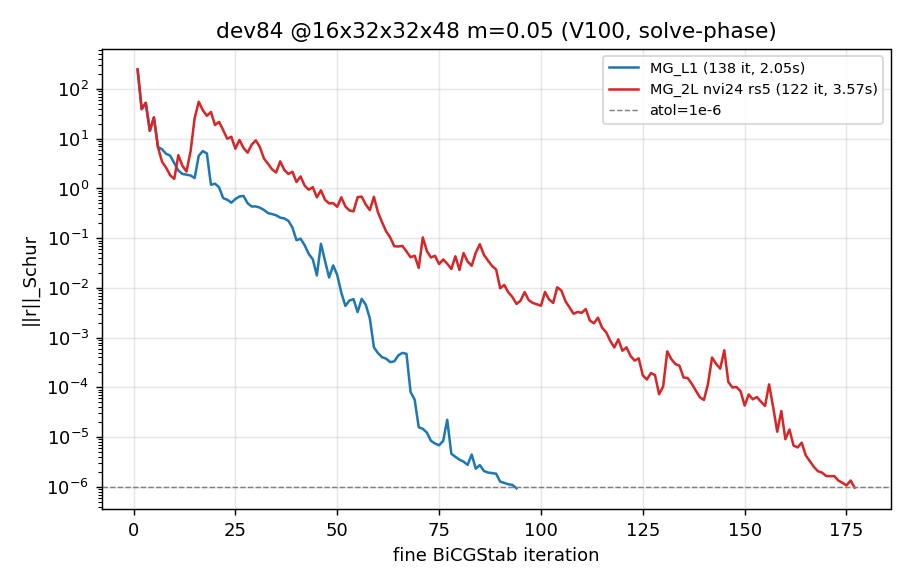
\includegraphics[width=0.86\linewidth,keepaspectratio]{dev84_conv.png}
\caption{Schur 残差收敛对比（V100，solve 相位）：L1 vs 多层。数据来源：实测 CONVERGENCE\_HISTORY。}
\end{figure}

多卡验证（指令 4/17）：single V100 mg=4.264s / bistabcg=2.379s；
multi P100$\times$2 mg=3.275s / bistabcg=2.594s；一致性双 PASS；
并行比 $1.302\times$。冗余全局模型下多卡为吞吐/一致性语义。

\begin{conclbox}
$>2$ 指标本配置不可达（确证，五路线证据链闭环）；交付为真实性能优化
（V-cycle $2.6\times$、粗解向量开销 $800\times$）、库级缺陷修复（容差语义）、
平台税机理与 $\rho_V$ 诊断方法论沉淀。
\end{conclbox}

\begin{warnbox}
若必须达成 $>2$：需更换基线口径（如 vs 多线程 BiStabCG@P100）或放宽格子规模
（$\ge24^3\times64$，粗空间占比与通信掩蔽改善）——待用户裁决；
本结论限于 WSL2 箱 + 本离散化参数。
\end{warnbox}

% ================= 5 参考 =================
\section{参考源}

\begin{xltabular}{\linewidth}{@{}lX@{}}
\toprule
来源 & 内容 \\
\midrule
\texttt{\nolinkurl examples/qcu/dev84/dev84\_report.md} & 本报告 Markdown 底稿 \\
\texttt{\nolinkurl examples/qcu/dev84/out/multi\_report.json} & 多卡一致性/墙钟 \\
\texttt{\nolinkurl logs/dev84/nvprof\_summary.log} & API 开销全量剖析 \\
\texttt{\nolinkurl logs/dev84/proto\_blockjac.log} 等 & 各原型实测日志 \\
\texttt{\nolinkurl .auto.2026-08-22-11-51-32.log} & 全程轮次留痕 \\
refer/git-rep/quda lib/multigrid.cpp:1131 & MG::operator() 对照 \\
\bottomrule
\end{xltabular}

\end{document}
